
% asset_id: FAS1VectorsTikZ-005
% asset_type: tikz
% topic_id: FAS1Vectors
% unit_code: FAS1
% topic_code: FAS1-VEC
% related_lesson_file: FAS1_vectors_lesson.md
% related_lesson_section: # 9. Visual Asset Integration
% source: FP1-Chp1-Vectors.pdf + transcripts.md where relevant
\documentclass[tikz,border=8pt]{standalone}
\usepackage{amsmath}
\usepackage{xcolor}
\usetikzlibrary{arrows.meta,calc,positioning}
\definecolor{Canvas}{HTML}{FAF9F6}
\definecolor{Ivory}{HTML}{FFFFF0}
\definecolor{LineGrey}{HTML}{E5E5EA}
\definecolor{Gold}{HTML}{C5A059}
\definecolor{TextInk}{HTML}{2C2C2E}
\definecolor{SoftPink}{HTML}{FBEFEF}
\begin{document}
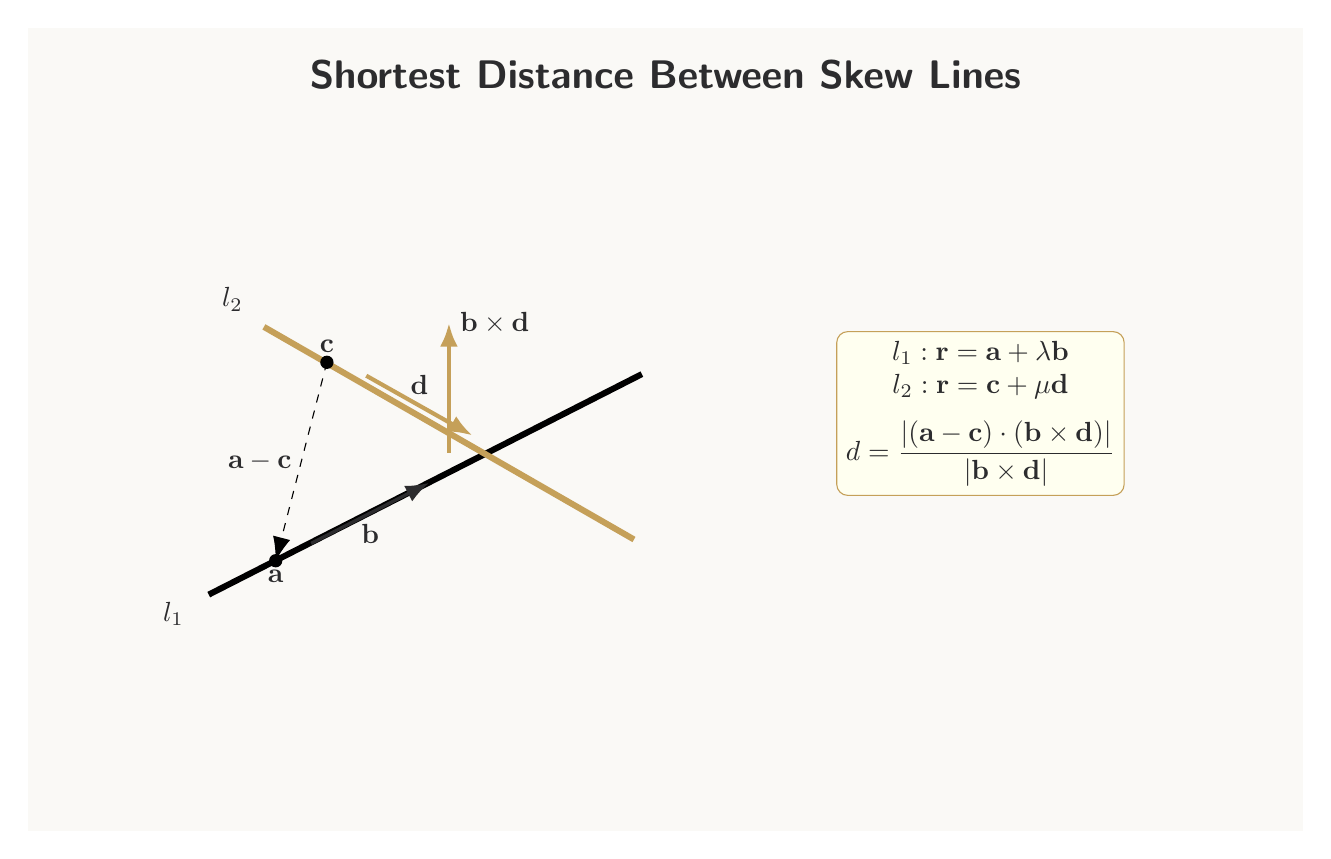
\begin{tikzpicture}[every node/.style={font=\sffamily,text=TextInk},arrow/.style={-{Latex[length=3mm]},line width=1.2pt,draw=TextInk},goldarrow/.style={-{Latex[length=3mm]},line width=1.5pt,draw=Gold}]
\fill[Canvas] (-0.6,-0.6) rectangle (15.6,9.6);

\node[font=\sffamily\bfseries\Large] at (7.5,9) {Shortest Distance Between Skew Lines};
\draw[line width=2.2pt] (1.7,2.4)--(7.2,5.2); \draw[Gold,line width=2.2pt] (2.4,5.8)--(7.1,3.1);
\node at (1.25,2.15) {$l_1$}; \node at (2.0,6.15) {$l_2$};
\draw[arrow] (3.0,3.05)--(4.5,3.82) node[midway,below] {$\mathbf b$}; \draw[goldarrow] (3.7,5.18)--(5.05,4.42) node[midway,above] {$\mathbf d$};
\fill (2.55,2.83) circle (2.4pt) node[below] {$\mathbf a$}; \fill (3.2,5.35) circle (2.4pt) node[above] {$\mathbf c$};
\draw[dashed,-{Latex[length=3mm]}] (3.2,5.35)--(2.55,2.83) node[midway,left] {$\mathbf a-\mathbf c$}; \draw[goldarrow] (4.75,4.2)--++(0,1.65) node[right] {$\mathbf b\times\mathbf d$};
\node[draw=Gold,fill=Ivory,rounded corners,align=center] at (11.5,4.7) {$l_1:\mathbf r=\mathbf a+\lambda\mathbf b$\\$l_2:\mathbf r=\mathbf c+\mu\mathbf d$\\[7pt]$d=\dfrac{|(\mathbf a-\mathbf c)\cdot(\mathbf b\times\mathbf d)|}{|\mathbf b\times\mathbf d|}$};

\end{tikzpicture}
\end{document}
